% Chapter Template
\chapter{The CMS experiment at the LHC} \label{Chapter2} 



This chapter outlines the main features of the Large
Hadron Collider (LHC) in Section~\ref{lhc} and of the Compact Muon Solenoid (CMS)
detector in Section~\ref{cms}. 



%----------------------------------------------------------------------------------------
%	SECTION 1
%----------------------------------------------------------------------------------------
\section{The Large Hadron Collider}\label{lhc}
The accelerator structure at CERN is a chain of machines that
progressively accelerate particles to higher energies. Before delivering the beam into the next stage in the succession, each machine
increments the energy of a beam of particles.\\
The Large Hadron Collider (LHC)~\cite{Brning2004LHCDR} –- the last step in this sequence –- is a circular particle accelerator
located at the CERN laboratories in Geneva operating since 10
September 2008. It is
designed to accelerate hadrons (like protons, Lead-ions, Xenon-ions) and to
operate at the centre-of-mass energy of 14\TeV.
The circular ring is installed in a tunnel of a 27 kilometers where
the Large Electron Positron collider~\cite{Lep:designReport} was
previously located. Several other accelerators in the succession have
their own experimental areas where beams are used for experiments at lower energies.
A graphic representation of CERN accelerator
complex is shown in Figure~\ref{fig:cern}. 

\begin{figure}[h]
\centering
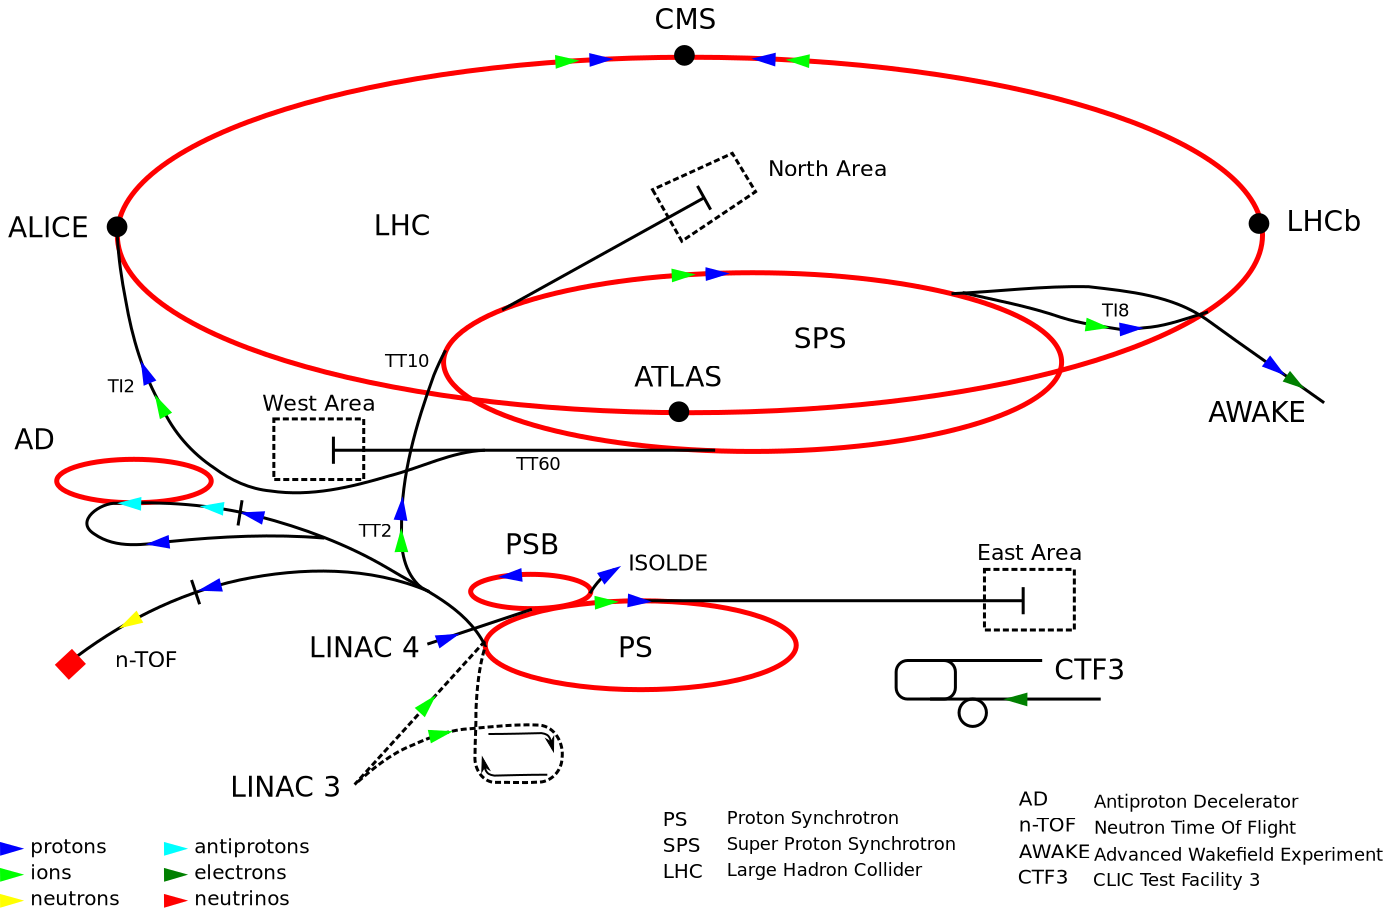
\includegraphics[width=0.75\textwidth]{Figures/c2/Cern-accelerator-complex.png}
\vspace*{3mm}
\caption{The LHC is the largest ring (top) in a complex chain of particle accelerators. The smaller machines are used in a chain to help boost the particles to their final energies and provide beams to a whole set of smaller experiments, which also aim to uncover the mysteries of the Universe~\cite{Mobs:2197559}}
\label{fig:cern}
\end{figure}

The LHC consists of accelerating components as well as
superconducting magnets to focus the hadrons, keep them on the right
trajectory and squeeze them tight together right before the
collision point. 
The protons are accelerated in opposite directions in two distinct
accelerator tubes which cross at four interactions points where the
protons are made to collide. At each of the interaction points along the ring,
four experiments are located with the aim to reconstruct the
sub-atomic particles made at the moment of the high energy collision.
The protons are grouped in bunches which are
accelerated in steps using the full accelerator chain consisting in a linear
accelerator, boosters, synchrotrons and, at the end, they are injected
into the LHC with an energy of 540\GeV. In the LHC ring, a system of
superconducting magnets further accelerate them up to 6.5\TeV (7\TeV)
to achieve a centre-of-mass energy of 13\TeV (14\TeV). Every
25 ns collisions between proton bunches occur meaning 40 million
bunch crossing per second. At full regime during data taking time
period about 2800 bunches travel in the LHC rings and each bunch is
made of up to $1.1\times10^{11}$ protons.

The four experiments located at the four interaction points are
ALICE~\cite{alice_2008} (A Large Ion Collider Experiment),
ATLAS~\cite{atlas_2008} (A Toroidal LHC ApparatuS),
CMS~\cite{cms_2008} and LHCb~\cite{lhcb_2008} (Large Hadron Collider
beauty) (refer to Figure~\ref{fig:cern}).\\
 ALICE experiment is designed
to study the presence and the properties of the hypothetical
quark-gluon plasma formed during heavy ions collisions, LHCb is
designed to be very sensitive in analyzing the properties of the B
mesons. The last two, ATLAS and CMS are general purpose detectors
designed to investigate a vast range of physics scenarios starting
from the search and discovery of the Higgs boson as far as exotic
searches for extra dimensions
and dark matter. \\

There are a few parameters which are accelerator-dependent but worth
mentioning because are also very important for the
physics analyses. They are the instantaneous and integrated luminosity, the
number, in the same bunch crossing, of simultaneous collisions and the
center-of-mass energy of the proton-proton collisions.\\
The instantaneous luminosity is defined as a time dependent
parameter, $d\mathcal{L}/dt$, which correlates the number of collisions
($N$) in a certain amount of time ($t$) and the cross section of a
given process:
\begin{equation}
\label{eq:instalumi}
\frac{dN}{dt} \: = \: \frac{d\mathcal{L}}{dt}\sigma
\end{equation}

The unit of the instantaneous luminosity is $b^{-1}s^{-1}$, where 1
barn $= 10^{-24} \ cm^2$ and it depends on the number of bunches in
the proton beam, on the number of protons per bunch and on the beam
optics. \\
The integrated luminosity is the integral of the instantaneous
luminosity over time, and relates the cross section of a
given process to the number of events $N$ of that process:
\begin{equation}
\label{eq:intelumi}
\mathcal{L} \:=\: \int \frac{d\mathcal{L}}{dt} dt \: = \: \frac{N}{\sigma}
\end{equation}


\begin{figure}[h]
  \noindent
  \makebox[\textwidth]{
  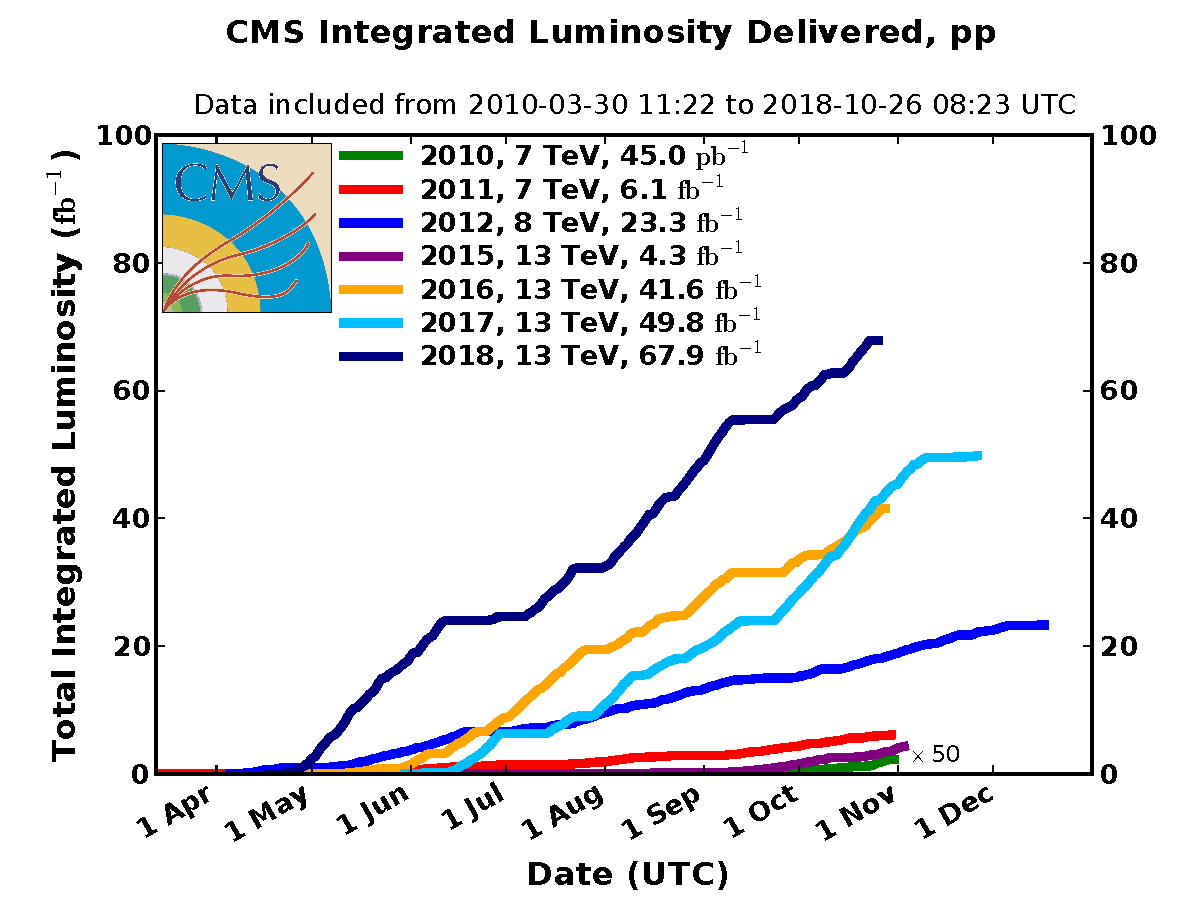
\includegraphics[width=.50\textwidth]{Figures/c2/int_lumi_cumulative_pp_2.pdf}
  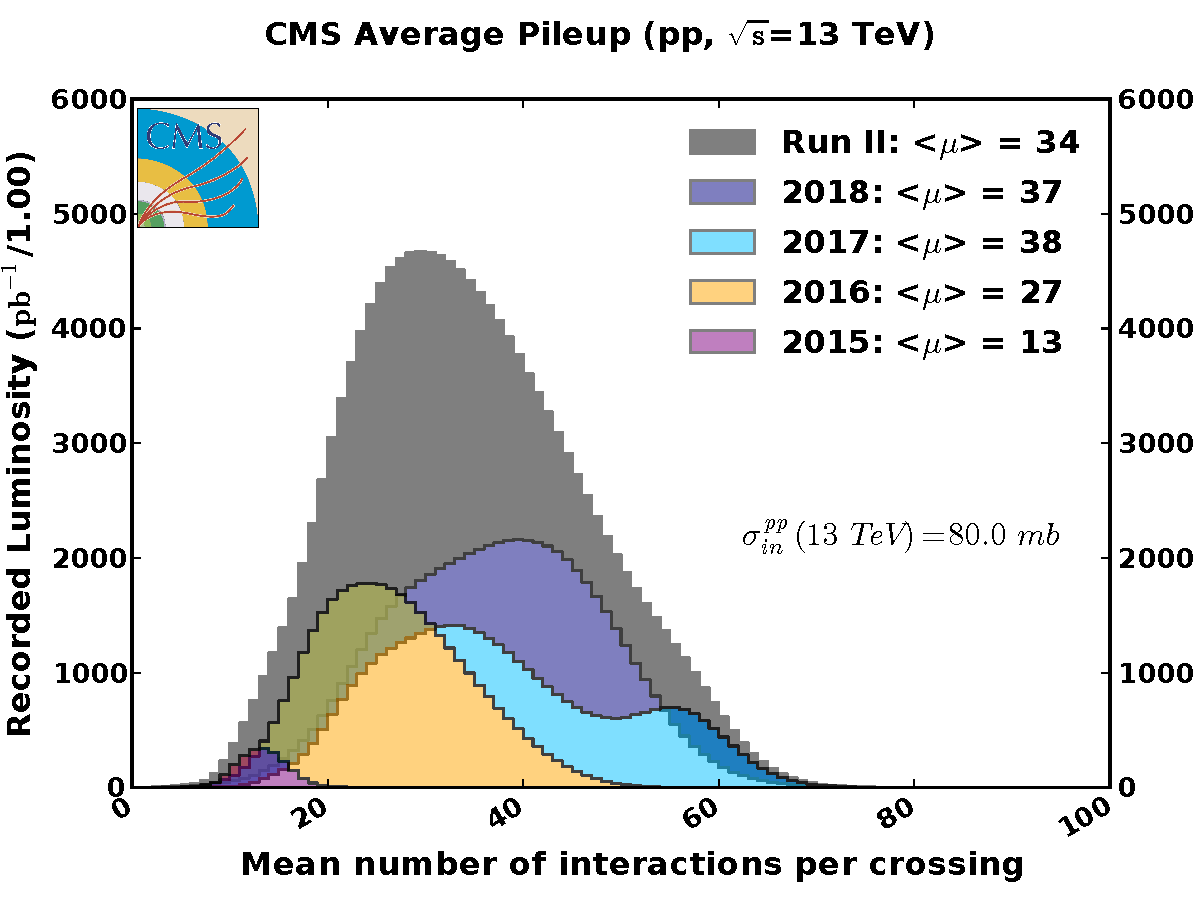
\includegraphics[width=.50\textwidth]{Figures/c2/pileup_allYears_run2.pdf}}\\
  \makebox[\textwidth]{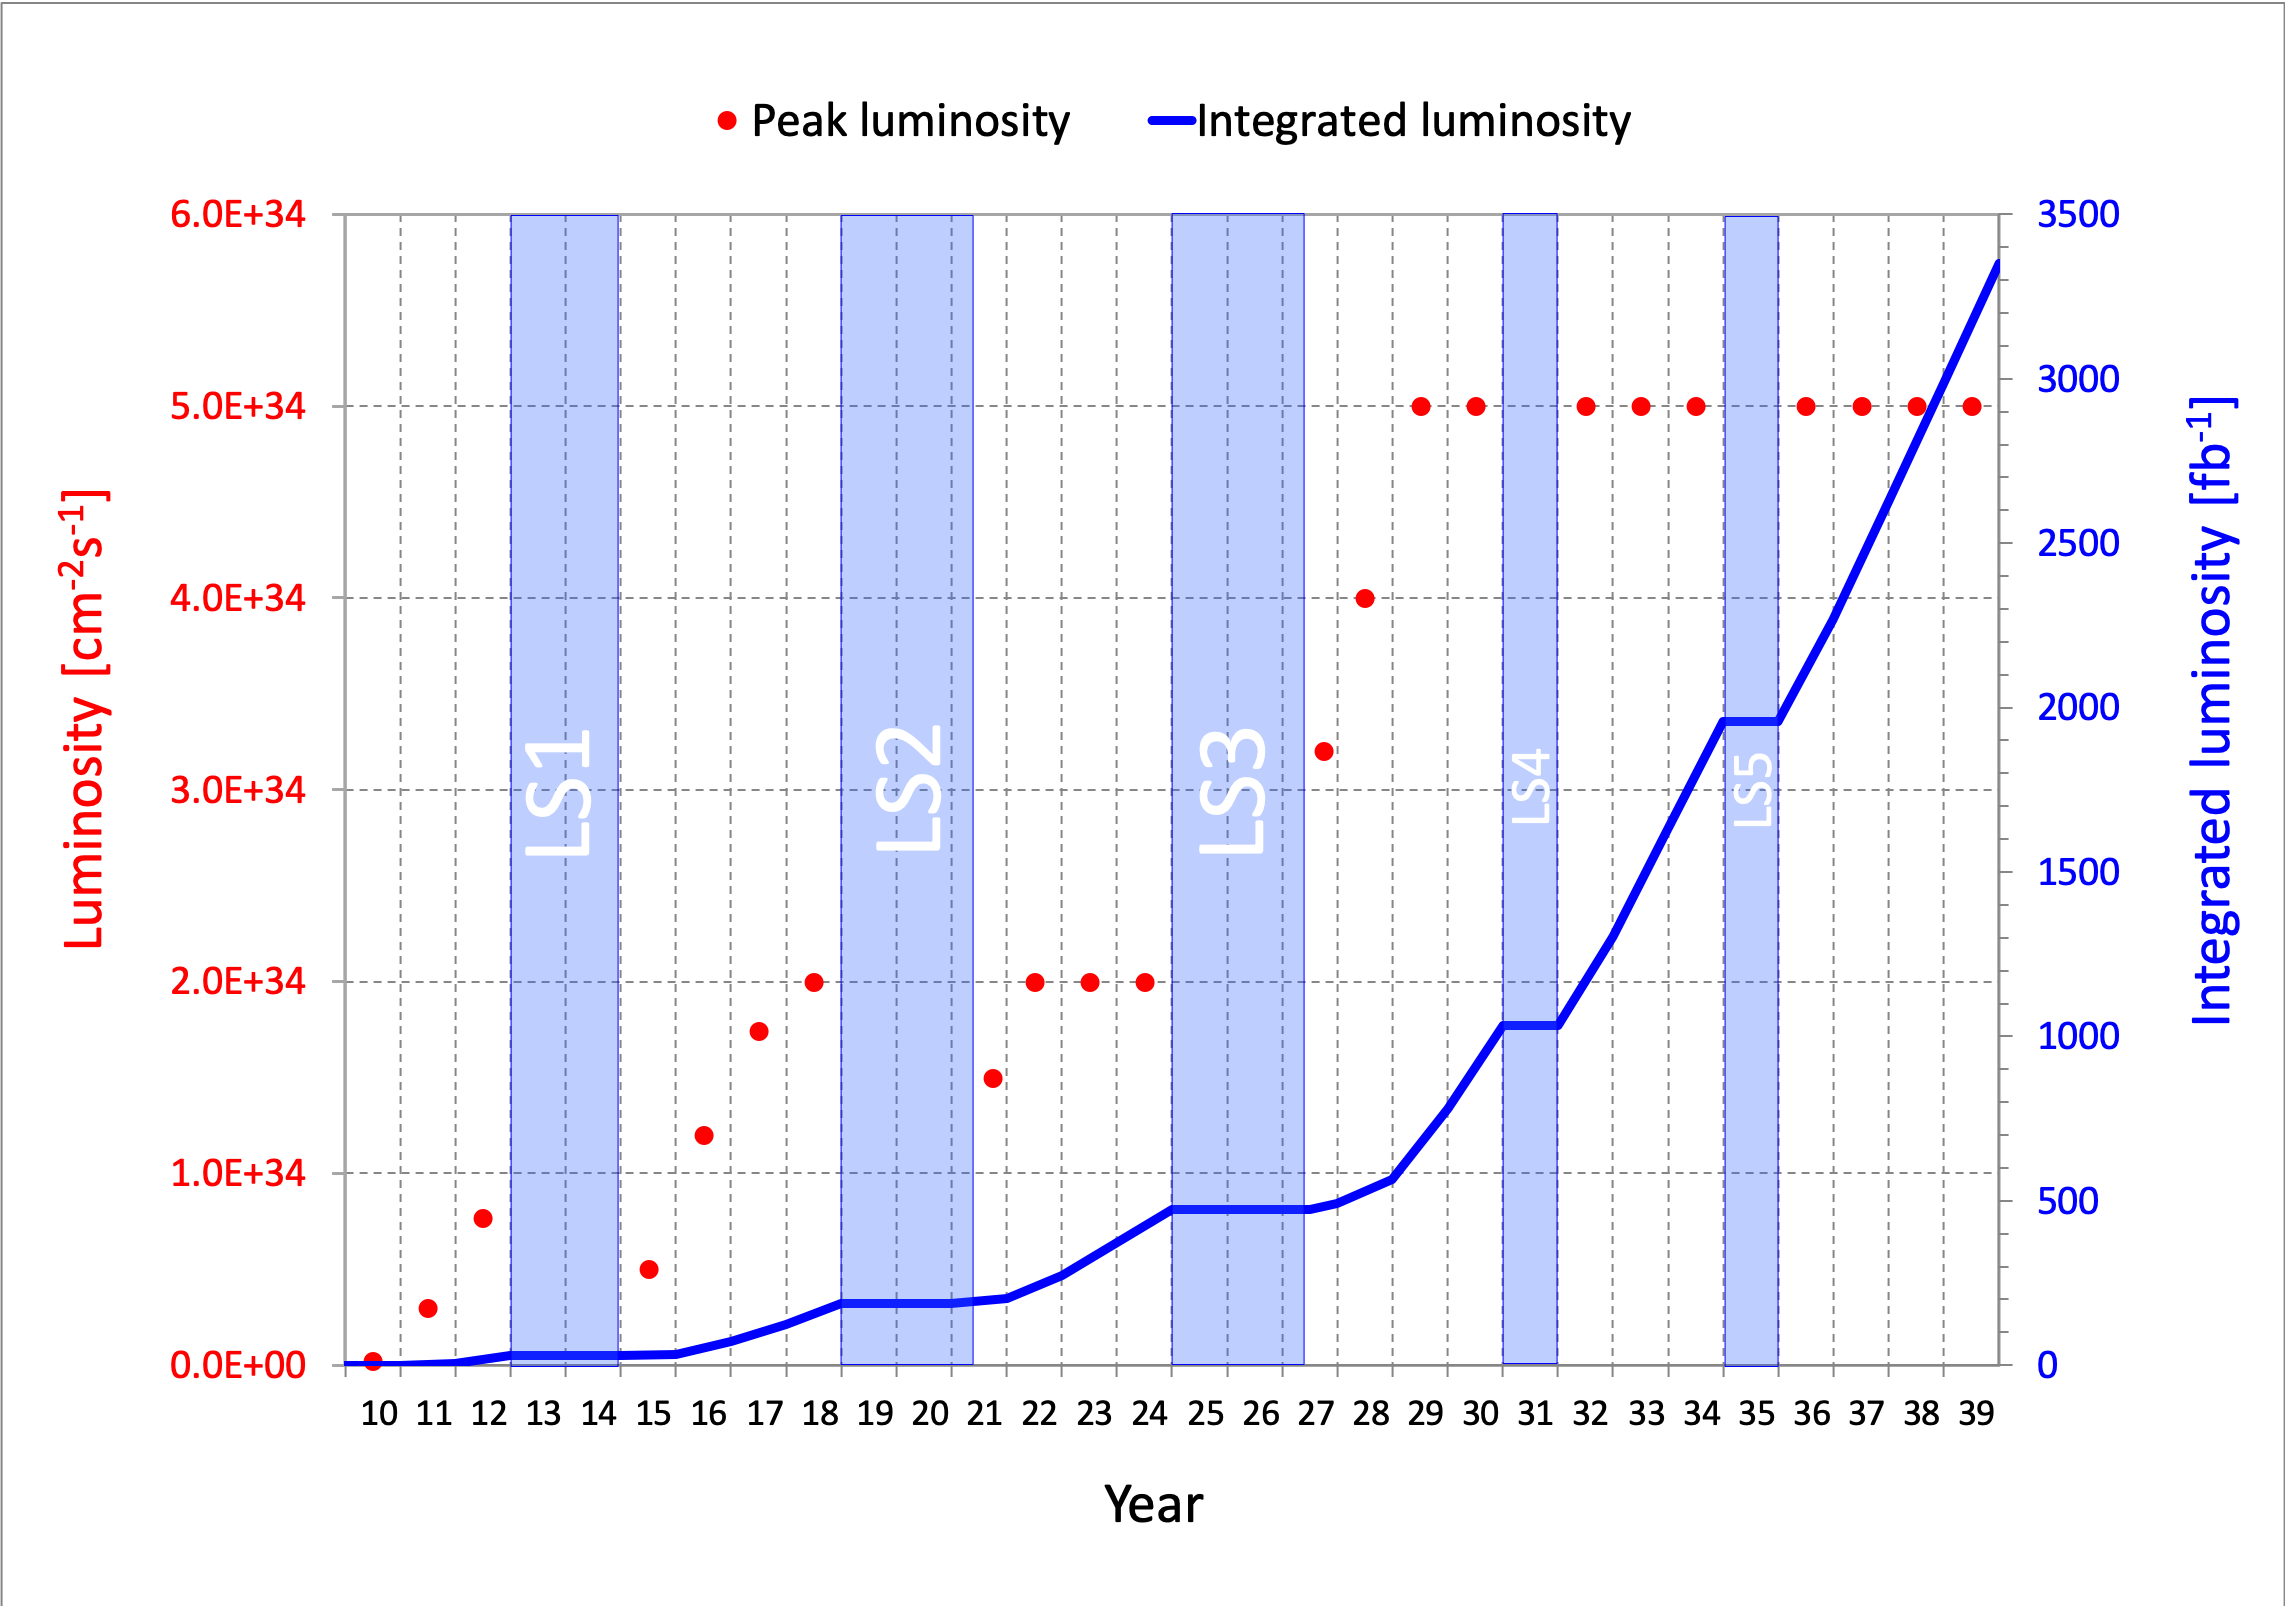
\includegraphics[clip,trim=0.2cm 0.2cm 0.2cm 0.2cm, width=.60\textwidth]{Figures/c2/Lumi.png}}
  \caption{Top-left: integrated luminosity delivered to the CMS
    experiment; top-right: distribution of the average number of
    interactions per crossing (pileup) for pp collisions in 2015
    (purple), 2016 (yellow), 2017 (azure), 2018 (periwinkle), and
    full Run2 (gray),~\cite{webpage_lumi}. Bottom: scheduled and
    projected integrated and instantaneous luminosity at the LHC~\cite{webpage_lhc}.}
  \label{fig:lumi}
\end{figure}

The LHC was designed to deliver an instantaneous luminosity
of $10^{34}cm^{-2}s^{-1}$.\\
Figure~\ref{fig:lumi} (top-left and central
plots) shows the schedule of the Large Hadron Collider from the start
to the following years of operations. The LHC has delivered two
outstanding runs of data taking: the first phase, Run1 (2010-2012) at
center-of-mass energy of 7 and 8\TeV and total delivered integrated
luminosity of $29.4\ fb^{-1}$; the first three years of data taking proved
the physics potentiality of the LHC with, among others, the Higgs boson
discovery. The second run, Run2 (2015-2018) started after two years Long
Shutdown when the machine and the detectors were 
consolidate to be able to run at the full capacity with 
center-of-mass energy of 13\TeV and total delivered integrated
luminosity of $162.9\ fb^{-1}$.\\
The increase in luminosity over the
years was the result of improvements in the beam quality and optics which
led to an higher number of pp collisions per bunch crossing. This
quantity is referred as pileup, PU which is shown in the top-right plot
in Figure~\ref{fig:lumi}. The average \textlangle{}PU\textrangle{} for
Run2 is 34. On one hand this large
number of collision per bunch crossing 
expands the physics reach of CMS and ATLAS because of
the higher probability of an episode of a rare collision; however
most of the PU interactions pollute the information of the
event being mostly soft and less interesting to look for
new physics models. Thus it is challenging for the detector and the for
the reconstruction algorithms to be able 
to disentangle and reconstruct each single pp collision per single
bunch crossing.

%-----------------------------------
%	SECTION 2
%-----------------------------------
\section{The Compact Muon Solenoid}\label{cms}

The Compact Muon Solenoid (CMS) detector is located at one of the four
collision points along the LHC ring, precisely at LHC P5 in Cessy in
France.  \\
CMS is a multi-purpose detector designed to observe any new physics
phenomena that could appear at proton-proton collision. CMS behaves
like a high-speed camera capturing instant frames of the particle
collisions up to 40 million times per second. Thus detector aims to recreate a
photograph of the collision by trying to
identify the particles created after the collision and
measuring their energies and momenta. \\
The idea behind the design was to create, around the place where the
two proton beams cross each-other, a structure of concentric cylindrical layers
in order to be able to track and measure the path of the particle
escaping from the center.   

\subsection{The CMS coordinate system} 
The coordinate system used by CMS is a right-handed system. It is defined
locating its 
\begin{wrapfigure}{r}{0.5\textwidth}
  \begin{center}
    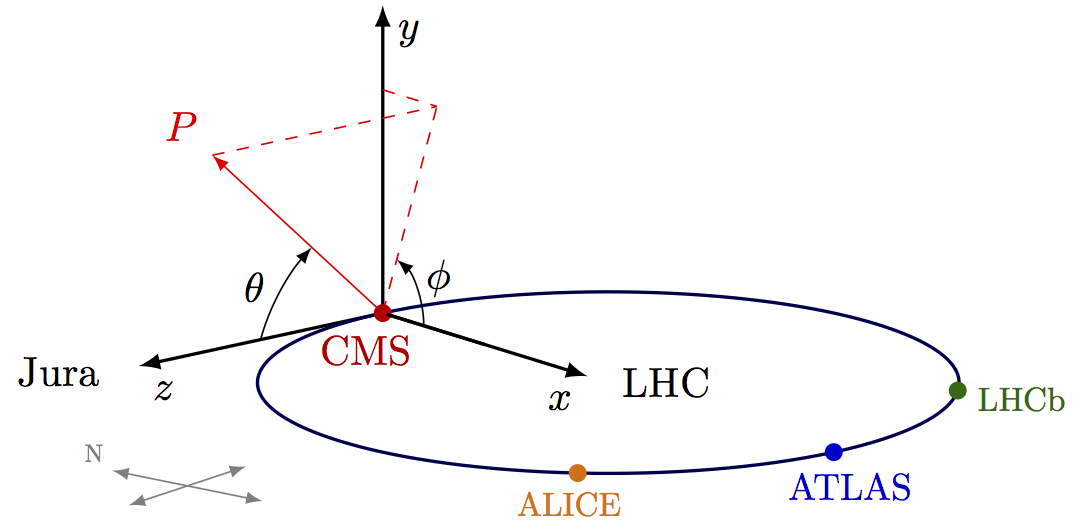
\includegraphics[clip,trim=0cm 0cm 0cm 0.1cm, width=0.48\textwidth]{Figures/c2/cms_coordinate_system.png}
  \end{center}
  \caption{A scheme of the coordinates system used by CMS~\cite{coordinate_cms}.}
\label{fig:coordinates}
\end{wrapfigure}
 center in the nominal interaction point, the
\emph{y}-axis is vertical pointing upwards, the \emph{x}-axis is
radial pointing inward towards the center of the LHC ring and the
\emph{z}-axis coincides with the direction of the beam
(counter-clockwise beam) (refer to
Figure~\ref{fig:coordinates}). The azimuthal angle $\phi$ is defined
from the \emph{x}-axis in the \emph{x-y} plane and the polar angle
$\theta$ is measured from the \emph{z}-axis in the same transverse
plane meaning \emph{x-y} plane.\\
For an object of energy $E$ and momentum $\overrightarrow{p}$,
rapidity, $y$ and pseudorapidity, $\eta$ are defined as:
\begin{equation}
\label{eq:pseudo}
y \: = \: \frac{1}{2} \ln \frac{E + p_z}{E - p_z} \;\; \approx \;\;
\eta \: = \: \frac{1}{2} \ln \frac{|\overrightarrow{p}| +
  p_z}{|\overrightarrow{p}| - p_z} \: = \: -\ln \tan (\frac{\theta}{2})
\end{equation}
The approximation of the rapidity with the pseudorapity is possible for
relativistic particles with $p_{T} \gg m$. The rapidity is used to
measured the angular distance between particles, $\Delta R =
\sqrt{\Delta y ^2 + \Delta \phi ^2}$ which is Lorentz invariant under
boots along the beam direction. With the prior approximation,
the $\Delta R$ quantity is often defined as $\Delta R =
\sqrt{\Delta \eta ^2 + \Delta \phi ^2}$.\\
Finally, using the $x$ and $y$ components, the transverse variables
are defined: the transverse momentum, $p_T$ and the transverse energy,
$E_T$.\\

The schematic representation of the CMS detector and its parts is
shown in Figure~\ref{fig:detector}


\subsection{CMS detector}\label{sec:cmsdetector}
\begin{figure}[h]
\centering
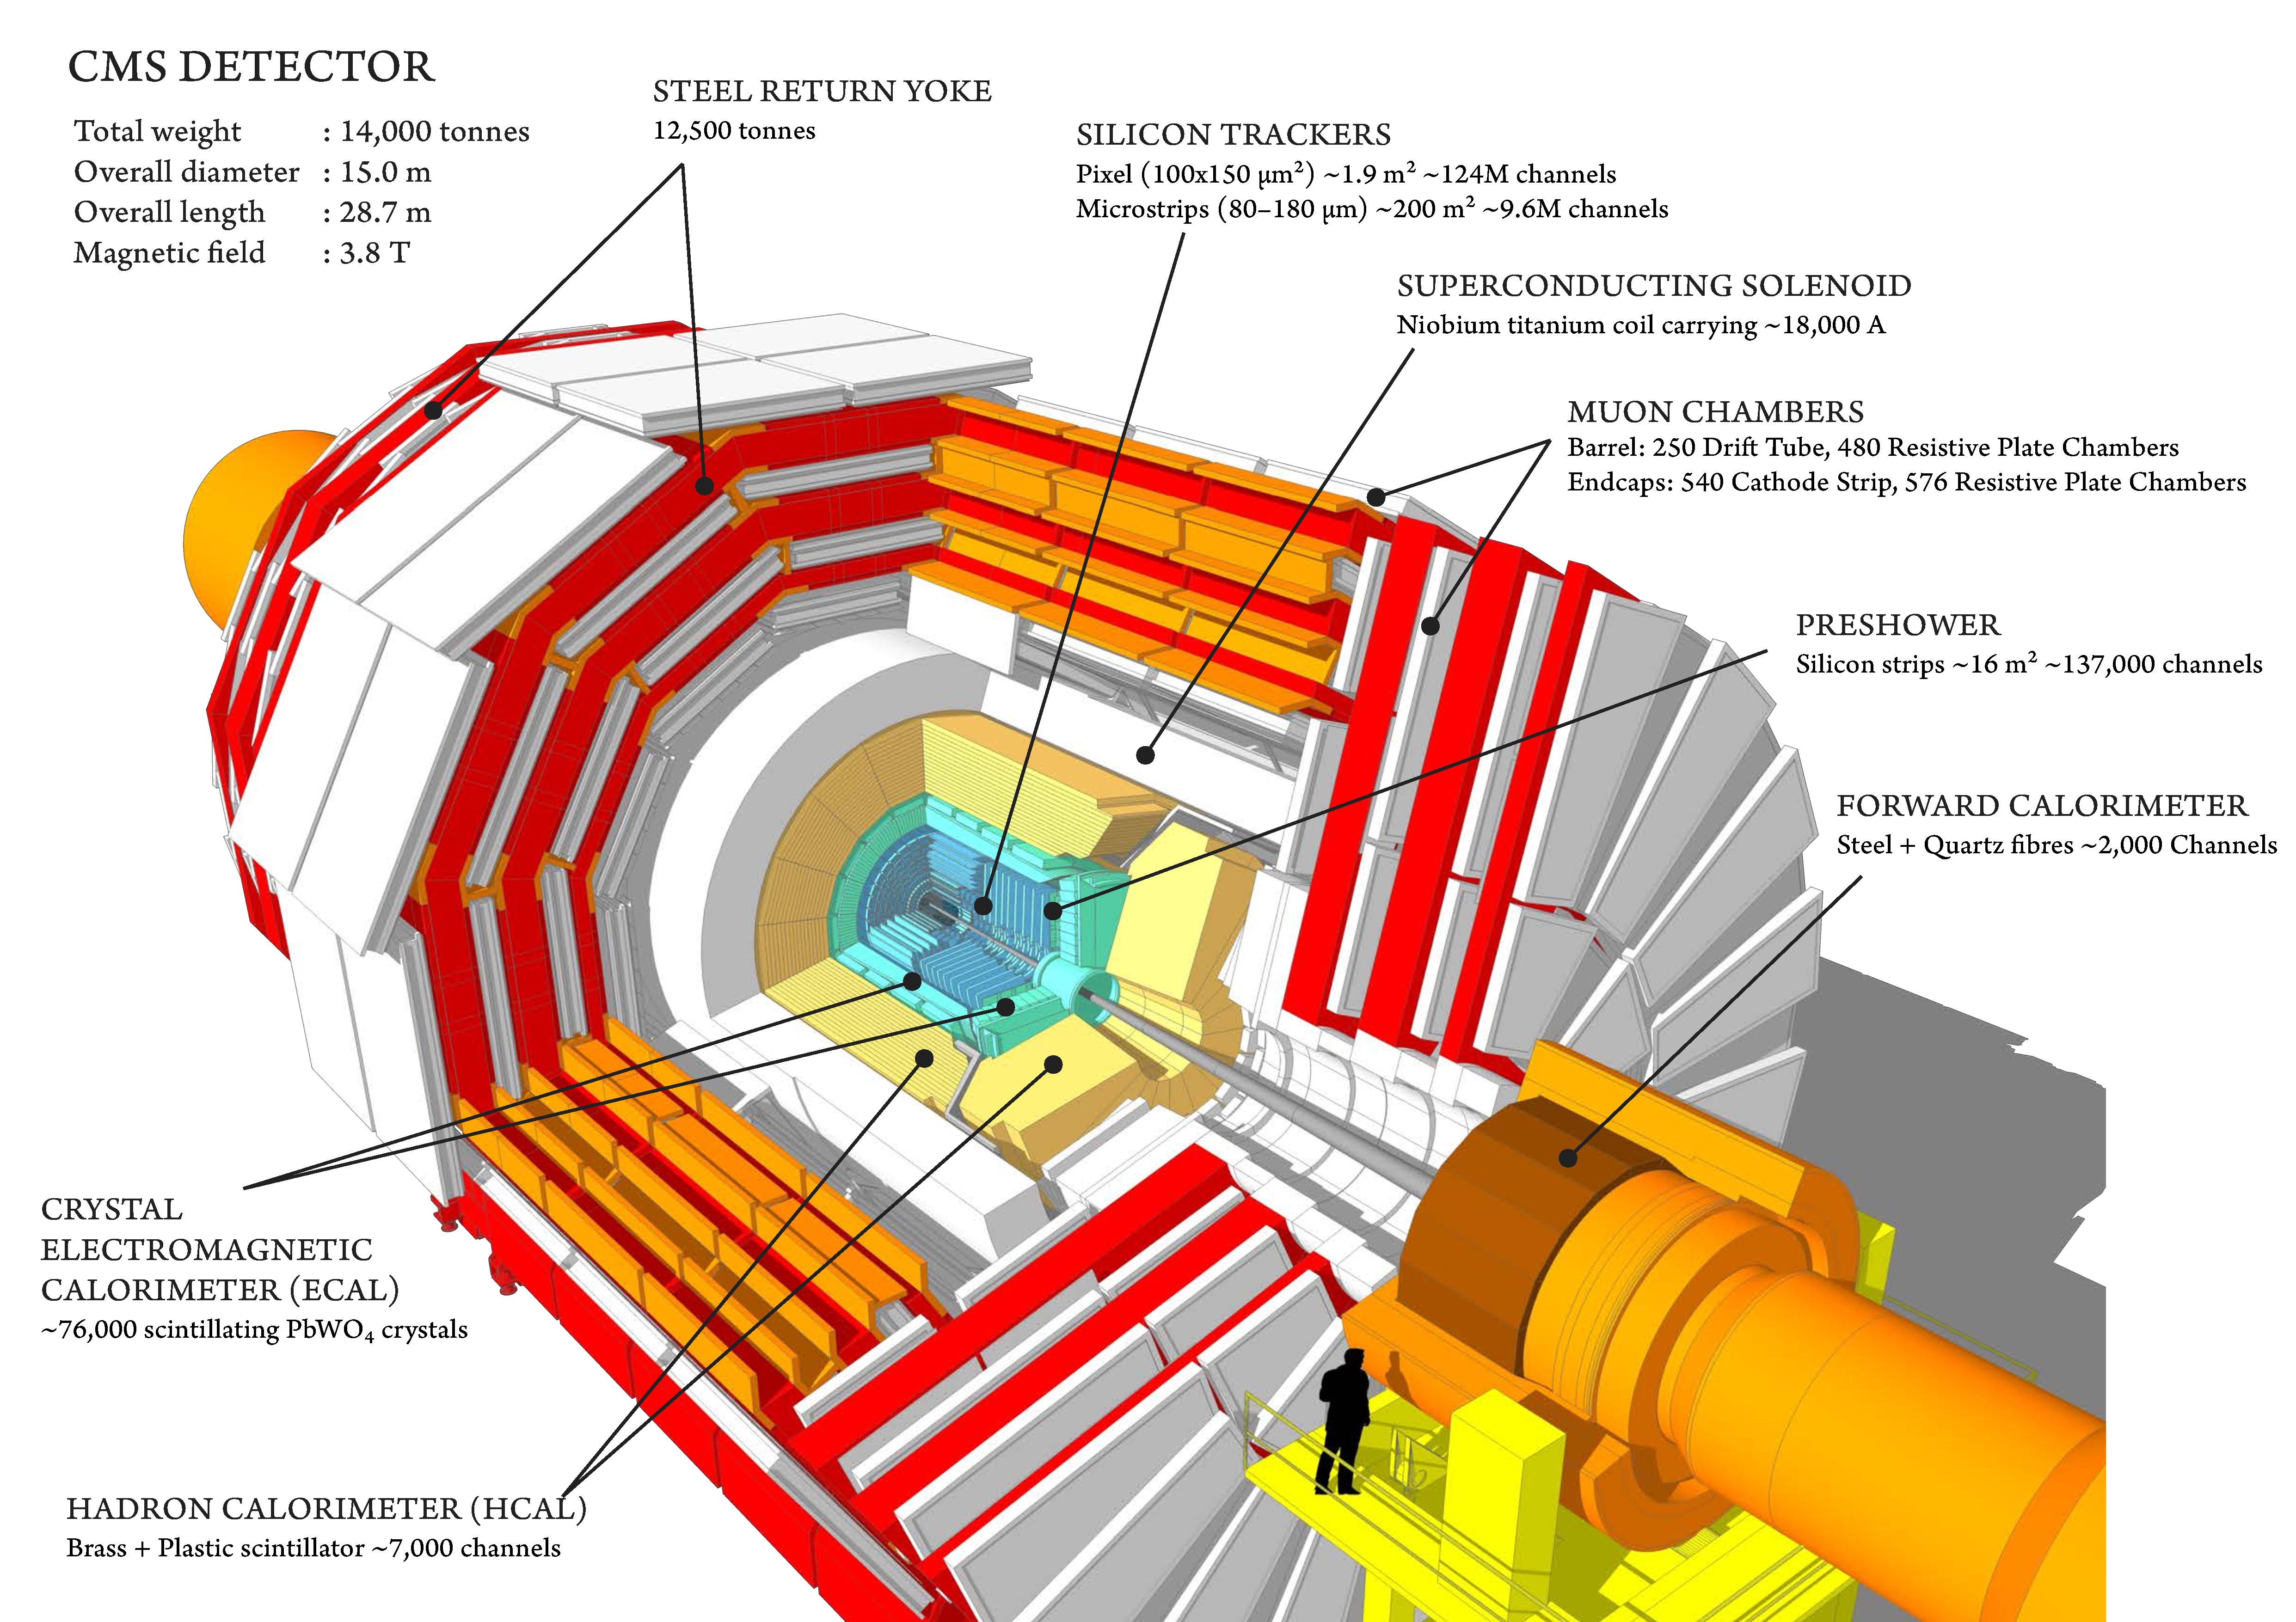
\includegraphics[width=0.98\textwidth]{Figures/c2/cms_160312_06-compressed.pdf}
\vspace*{3mm}
\caption{A scheme of the CMS detector and its parts~\cite{webpage_cms}.}
\label{fig:detector}
\end{figure} 
With CMS detector is possible to measure photons, electrons, muons and hadrons (neutral and charged). 
To be able to achieve such results, CMS is made of a system of sub-detectors each of which contributes with
measurements of specific properties and quantities of different 
particles. The overlap and combination of all the
informations from the sub-detectors allow to identify and measure the
properties of the particles produced during the collision~\cite{CMS:particleflow}. Beginning
with the region at the immediate proximity to the interaction point, a
particle meets first the tracker where its trajectory, if charged, is
measured. This measure is possible thanks to the presence of the
magnetic field, created by the solenoid, which bends the charge
particle tracks. Subsequently there are the
electromagnetic (ECAL) and hadronic (HCAL) calorimeters where
electrons/photons and hadrons are receptively absorbed and their
energies measured. Finally the muons, getting through the
calorimeters, enter into the muon chambers where the whole trajectories
are measured~\cite{CMS:particleflow}. The full reconstruction
procedure is explained in the following Chapter~\ref{Chapter2_5} in Section~\ref{sec:reconstruction}.\\

The subsystems of the CMS experiment are listed and briefly described
in the following paragraphs.

\subsubsection{The superconducting solenoid}
The central part of CMS is a solenoid magnet of 6 m internal diameter
which is made of a cylindrical coil of superconducting fibers. It 
provides a magnetic field of 3.8 T. 
\subsubsection{The tracking system}\label{sec:tracking}
The particle energy measurement is a critical information to build up the full
picture of the event happening at center of CMS detector. One way to
estimate the momentum is to track the particle course through a
magnetic field; the more bent the trajectory, the less energy the
particle has. The CMS tracking system registers the course taken by
charged objects passing through by spotting their location at a few
fixed points which are the tracker layers. \\
Thus the system can measure the trajectories of muons, electrons,
charged hadrons and tracks originating from the secondary vertex decay of long-lived
particles.

The tracker modules need to have relative fast responses, good
accuracy as well as be lightweight in terms of radiation lengths in
order to disturb the particle path as little as possible. Furthermore
the layers closer to the beam pipe receive
the largest volume of particles thus the construction materials should
have high radiation hardness to resist radiations over time.

Hence the design of the CMS tracking system is optimized to
efficiently and precisely measure the trajectories of charged
particles and to effectively reconstruct secondary vertices.\\
This latter feature is of particular
importance in the context of displaced vertices search presented
in Chapter~\ref{Chapter6}. The vertex position resolution and track
reconstruction efficiency play a major role in the analysis acceptance,
and thus in the analysis sensitivity. Those parameters are going to be
described in detail in Section~\ref{sec:trackvertex}.

\begin{figure}[h]
\centering
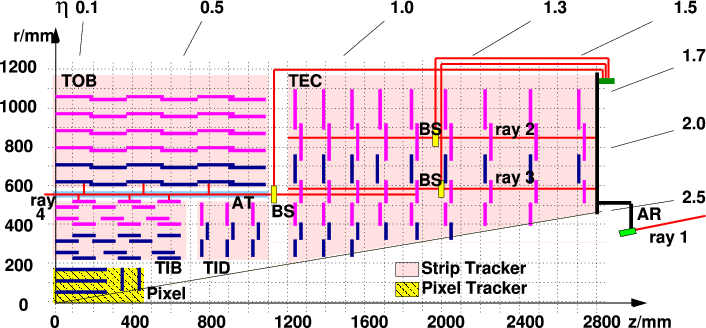
\includegraphics[width=0.98\textwidth]{Figures/c2/las}\\
\vspace{1cm}
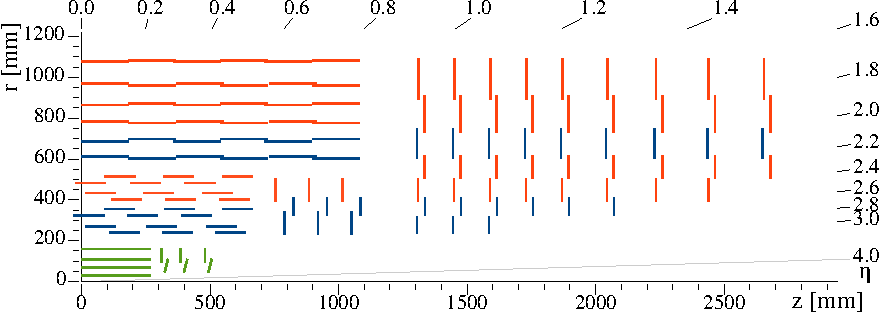
\includegraphics[width=0.78\textwidth]{Figures/c2/Phase1_Tracker_1Quarter.pdf}

\caption{Top: a quarter of the CMS silicon tracker in an $r-z$
  view. The strip tracker comprises several parts: the tracker inner
  barrel (TIB), outer barrel (TOB), inner disks (TID) and endcaps
  (TED)~\cite{Adam:1171503}. Bottom:
sketch of one quarter of the current CMS tracking system in
  r-z view, 2017-2018 data taking. The pixel detector is shown in
  green with the additional modules~\cite{trackingPU}.}
\label{fig:tracker}
\end{figure} 
Additionally the tracking system exhibits high granularity and
fast response features to correctly associate each reconstructed track
to the respective bunch crossing and the primary interaction vertex.

The CMS tracker consists of a pixel detector (pixel Tracker) and a
silicon strip detector (strip Tracker), see
Figure~\ref{fig:tracker}. While a particle travels through the tracker the pixels and
strips create very small electric signals which get amplified and
detected.\\
The original pixel detector was made of three barrel
layers at radii of 4.4, 7.3, and 10.2 cm and two endcaps modules in
the forward region. 
During the short shutdown between the data takings 2016 and 2017, it
was installed an
upgraded version of the pixel detector. The detector has currently four
barrel layers at radii of 3.0, 6.8, 10.2, and
16.0 cm and three layers in the forward region~\cite{Dominguez:1481838}. The
recent innermost layer and modules
are positioned closer to the beam pipe in order to improve the
precision on the position of the interaction vertices.\\
The silicon strip detector consists of many parts: the tracker inner and
outer barrels (TIB and TOB), in total ten layers of strip modules in
the barrel; the 6 tracker inner disks (TID), three each
side; and the nine disks on each side of the tracker endcap (TEC).\\
In total the tracking system is 5.8 m long and 2.6 m high,
extending the coverage of the tracker up to $|\eta|$ = 2.5. The total
amount of sensors is 66 million for the pixel and 124 million for the
strip detector. 

\subsubsection{The electromagnetic calorimeter}
The ECAL detector is a fine-grainded and homogeneous calorimeter
made up of lead
\begin{wrapfigure}{r}{0.6\textwidth}
  \begin{center}
    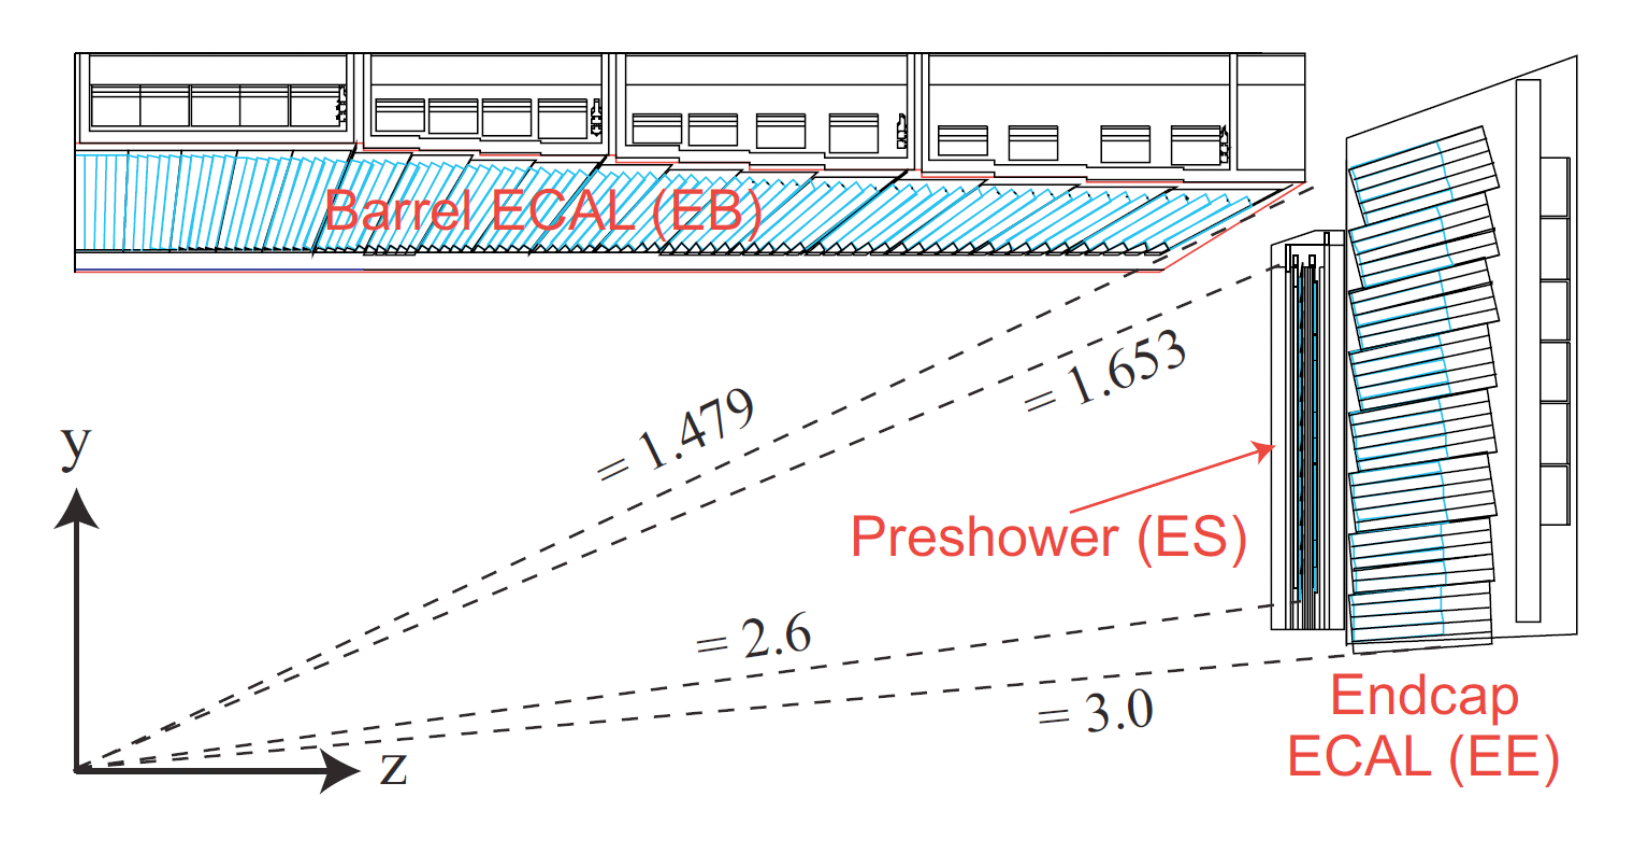
\includegraphics[clip,trim=1cm 1cm 1cm 1.5cm, width=0.58\textwidth]{Figures/c2/ecal}
  \end{center}
  \caption{Geometric view of one quarter of the ECAL~\cite{Benaglia_2014}.}
\label{fig:ecal}
\end{wrapfigure}
 tungstate crystals. Those single crystals are extremely transparent
 and \emph{scintillate} when photons and electrons pass through
 them. \emph{Scintillation} occurs when in an excited atom, after given
 energy, an electron which went to an higher orbit falls back and
 releases energy in the form of a photon. The CMS ECAL's crystals
 receive energy from the showers of electrons, positrons and photon
 generated from the interaction between high energy photons/electron and
 dense matter. Afterwards the crystal atoms ``relax'' and each
 excited electron, ``falling back'',
 emits energy as a photon in the blue light spectrum.
The light produced is proportional to the particle's energy
 allowing a fast and very precise measurement of the momentum
 property. 

The single crystal length in barrel region is 230 mm (220
 mm in endcap) comparable to $\sim$26 (25) radiation lengths meaning it
 absorbs more than 98\% of the energy deposited by the particle~\cite{Biino_2015}.\\
A scheme of the ECAL is shown in Figure~\ref{fig:ecal}.
ECAL modules are placed in the barrel ($\eta<$ 1.479) and endcap
(1.635 $<\eta<$ 3.0) regions, and a preshower detector is located just
before the endcap crystals. The preshower detectors help CMS to
distinguish between single high-energy photons and the less
interesting pairs of low-energy photons very close to each other, \ie
coming from the decay of a $\pi^0$. \\
For the analyes presented in Chapters~\ref{Chapter5}
and~\ref{Chapter6} the electron energy correctness is crucial for the
proper electron reconstruction and identification in the final
state. 

\subsubsection{The hadron calorimeter}
The HCAL detector is a hermetic sampling calorimeter which means it
consists of alternative layers of ``absorber'' and ``scintillator''
materials that measure a particle’s position, energy and arrival time.
At the moment a hadron collides with a absorber layer, brass or steel
in this case, an interaction occurs generating several secondary
particles. Subsequently these bunch of particles hit a successive layers
of absorber interacting again and agin and creating a shower of particles.
This shower passes through the layers of scintillators
causing them to emit photons in the blue-violet light spectrum.
The quantity of light in a given position is summed up over several
layers of tiles in depth, called a “tower”, thus this total amount of
light is a measure of a particle’s energy.\\
The HCAL is located both inside the solenoid, the main part, and
outside it, the outer barrel (HO). 
Inside the magnet coil, the barrel (HB) and endcap parts (HE) cover
respectively the pseudorapidity
ranges $\eta<$ 1.3 and 1.3 $<\eta<$ 3.
The forward region of pseudorapidity is covered by the forward hadron
calorimeter (HF) up to $\eta<$ 5. It is made up of iron radiators and
quartz-fibre sensors and it measures both the electromagnetic and the hadronic shower. 
The outer barrel, HO, ensures no energy leaks out the
back of the HB undetected.

\subsubsection{The muon system}\label{sec:muonsystem}
The muon system is constructed to detect muons and to measure their
trajectories. Muons can be created in the decay of numerous particles,
like Higgs Boson decay ($H \rightarrow \mu \mu \mu \mu$) or 
RH neutrino decay as described in
Chapters~\ref{Chapter4}, ~\ref{Chapter5} and~\ref{Chapter6}. For this
reason they
appear to be one of the clearest and golden ``signatures" for many
searches becoming the crucial element of the CMS reconstruction
and identification.\\
Since the muons can penetrate various meters of iron in the CMS return
yoke without interacting, the modules to detect muons are located at
the very edge of the detector where they are likely the only particles
which are able to register a signal.\\
The muon system is composed by three different kind of gaseous particle
detectors inserted in the steel yoke. All three sub-detector are
based on the confined ionization of a small gas volume within the detector
module due to the transit of an ionizing particle.
There are the drift tubes
modules, DTs, the cathode strip chambers, CSCs and the resistive plate
chambers, RPCs.
The four layers of DTs are located in the barrel and they cover up to
$\eta<$ 1.2 pseudorapidity range in the detector. \\
The rates in the forward region are higher than in the
barrel region, so a faster detector is needed there; this is the
reason for the CSCs instead of the DTs (shorter drift distance than DTs).
The four layers of
CSCs are installed in the endcap covering the pseudorapidity range 0.9
$<\eta<$ 2.4. \\
A part from an optimal spatial resolution given by the CSDs and DTs
combination, the muon system is required to have a time resolution of
the order of 1 ns. This is accomplish by adding the RPCs in the system
which grant for almost univocal identification of the proper bunch
crossing and for excellent info of the time coincidence of track
segments (refer to Section~\ref{sec:trackvertex}) from the distinct
muon sub-modules. 
The RPCs are positioned both in barrel
and endcap parts up to $\eta<$ 1.6. The whole pseudorapidity range of
the muon system allow to measure muons up to $\eta<$ 2.4.

Combining both the great spatial resolution of DTs and CSCs and the
high time resolution from the RPCs,
 the CMS muon system exhibits two
complementary and crucial inputs for the trigger system. 



\begin{figure}[h]
\centering
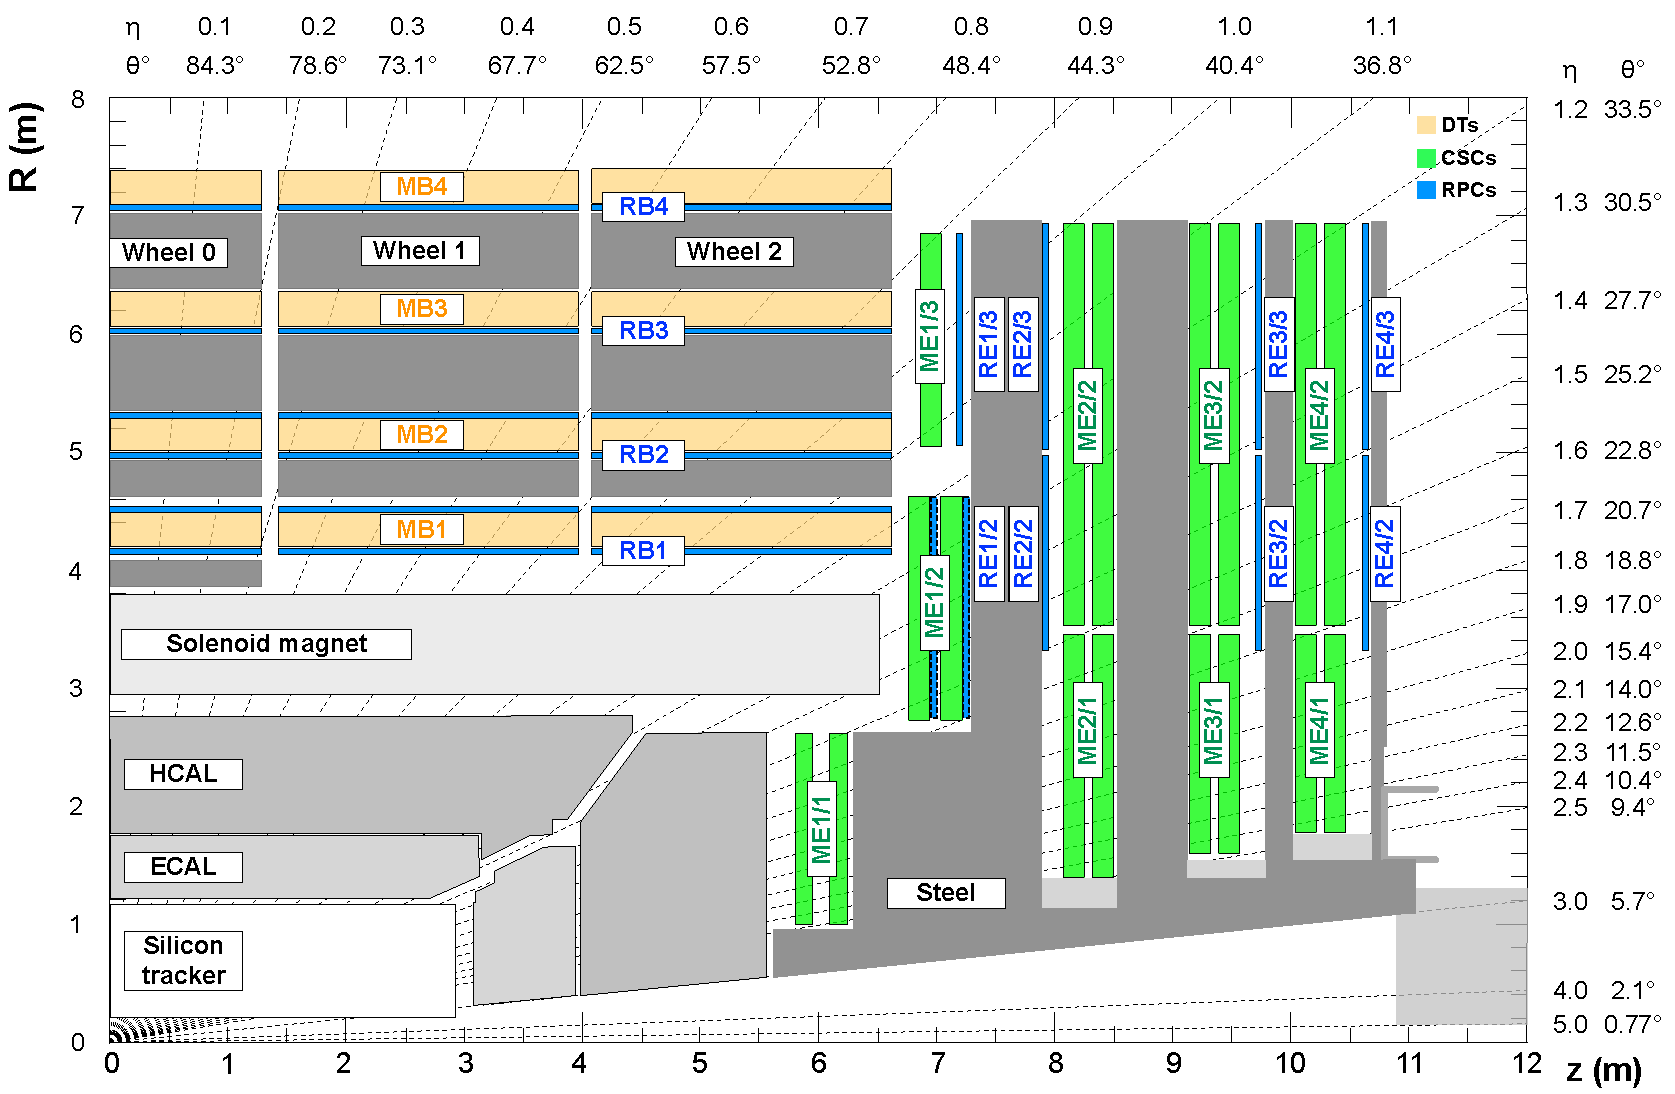
\includegraphics[width=0.98\textwidth]{Figures/c2/cms_quadrant_run_ii.pdf}
\caption{Geometric view of one quadrant of CMS. The grey areas are
  tracker, ECAL and HCAL systems; the colored
  areas show the muon system and its subsystem. The drift tube, DTs,
  modules are labelled MB (muon barrel) and the cathode strip
  chambers, CSCs, are labelled ME (muon endcap). Resistive plate
  chambers, RPCs, are labelled RB and RE and they are mounted in both the barrel and endcaps of CMS
~\cite{muonsystemPU}. }
\label{fig:muonsystem}
\end{figure} 

\subsubsection{The CMS trigger system}\label{sec:triggersystem}

At center of the CMS detector, proton-proton collisions occur every
25 ns which means a frequency of 40 MHz. However not every collision is
necessarily of potential interest for the CMS physics program and
moreover there are technical limitations on the rate the collision data can be
saved on disk to be analyzed offline. Thus a trigger is needed to be
able to sort between potentially interesting events and the extent of
inelastic scattering events.
Since the reading and storing time of the collision data is larger
than the collision frequency the viable solution is
to store the informations in pipelines that hold and process data
from several collision at the same time.
To work without mixing particles from two different events, it is
required that detectors have very good time
resolution and the signal from the millions of channels of different
systems to be synchronized and integrate.

The CMS trigger has a two-stage architecture~\cite{Khachatryan_2017}. The first level, L1 is
implemented in custom hardware and uses informations from the 
all muon systems and the calorimeters to identify events applying a fast
basic identification of measured particles. The first step reduces the
event rate to $\sim$100 kHz. The events sorted by the L1 are further refined by the
high-level trigger, HLT. It is a software farm that employs informations from all sub-detectors to perform a
refined event reconstruction reducing the rate down to a few kHz. The 
events are then saved for offline analysis.
The trigger selection is a irreversible process, what was not selected
by it is lost and it can not be recovered~\cite{Khachatryan_2017}.=

A complete sequence of L1
and HLT selection criteria, including any prescale, is referred to
as a trigger path.
%%%%%%%%%%%%%%%%%%%%%%%%%%%%%%%%%%%%%%%%%%%%%%%%%%%%%
\section{Summary}\label{sec:summaryC2}

In this chapter the LHC and CMS detector were presented.\\
We briefly introduced LHC timeline since 2010 and we listed the
reached values of instantaneous luminosity and center-of-mass energy
over the past years.
We illustrated that CERN accelerator chain produces
6.5 TeV proton beams circulating in the LHC tunnel and colliding in
four points one of which is the CMS detector. The data analyzed in
this work were collected over a three years period (2016-18) of the
LHC data-taking and coincide to an integrated luminosity of
137\fbinv.

We presented the CMS detector with all its sub-components and thes
trigger system.\\
We explored the detector subsystems: the tracker made up of pixel and
strip parts, the electromagnetic
and hadronic calorimeters and finally the muon system. For each of
those, we briefly list some details on the detection principle,
the geometry, and overall performances. \\

I have personally taken part in the 2017 data-taking while performing
shifts as RPC ``detector-expert-on-call''. This activity gave me the
opportunity to comprehend the complexity of the CMS detector in its
completeness. In the detector control-room located at P5, there is the
monitoring center of all detector inputs from the gas-mixtures
for the muon-system's sub-detectors to the cooling system of the
solenoid and the high voltage monitoring for the high powered
modules. At the same time the online performances of the different layers
are checked as the occupancy of the modules and the dead-time of each
detector. Simultaneously from the control room it is possible to oversee the LHC
delivered instantaneous luminosity, the related pileup number of
vertices and the L1 and HLT instant rates. \\
Being at P5 shows firsthand the importance of an attentive
data-taking for the subsequent data quality. All the electronic
signals recorded during each run are going to be stored as raw data
and then used for the offline event
reconstruction which is the subject of the next Chapter.